\documentclass[aspectratio=169, handout]{beamer}

\usetheme{metropolis}
\setbeamercovered{transparent}
\setbeamertemplate{navigation symbols}{}

\bibliographystyle{alpha}

\definecolor{unibsblue}{RGB}{60, 88, 155}
\definecolor{lightbeige}{RGB}{255, 251, 241}
\definecolor{textcolor}{RGB}{50, 50, 50}

\usepackage{cmbright}
\usepackage{subfig}
\usepackage{siunitx}
\usepackage[final]{graphicx}
\usepackage{pdfpages}

\graphicspath{{images}}
\usepackage[main=italian,english]{babel}
\usepackage[utf8]{inputenc}
\usepackage{csquotes}
\usepackage[T1]{fontenc}
\usepackage{hyphenat}

%\bibliographystyle{plain}
%\renewcommand{\bibname}{Bibliografia e Sitografia}

\usepackage[backend=biber,doi=false,isbn=false,mincitenames=1,maxcitenames=4,style=ieee]{biblatex}
\DeclareFieldFormat{sentencecase}{#1} % never apply sentence casing, even if bibtex field is unprotected
\DeclareFieldFormat{titlecase}{#1} % never apply title casing, even if bibtex field is unprotected
\addbibresource{./biblio/datasheets.bib}
\addbibresource{./biblio/refs.bib}
\addbibresource{./biblio/sites.bib}
\addbibresource{./biblio/images.bib}


\title[Relazione Finale]{Sviluppo di un sistema di supporto alla programmazione per dispositivi integrati della famiglia AVR}
\author[S.Fontana Matr. 727199]{Stefano Fontana}
\date{2021/2022}
\makeatletter 
    \newcommand{\insertrawshotauthor}{\beamer@shortauthor} 
    \newcommand{\insertrawshorttitle}{\beamer@shorttitle} 
    \setlength{\metropolis@frametitle@padding}{3.5ex}% <- default 2.2 ex
\makeatother

\defbeamertemplate*{title page}{customized}[1][]
{
    \begin{center}
        
\includegraphics[width=.23\textwidth]{logo_unibs_40.png}

        DIPARTIMENTO DI INGEGNERIA DELL'INFORMAZIONE
        
        Corso di Laurea in Ingegneria Informatica
    \end{center}
    \vfill
    \begin{center}
        \insertshorttitle\\
        {\fontfamily{cmr}\fontsize{14}{27}\color{black}\selectfont\textbf{\inserttitle}}
    \end{center}
    \vfill
    \begin{minipage}{.48\textwidth}
        \textbf{Relatore:}\\
        Chiar.mo~Prof.~Alessandro~Depari
    \end{minipage}
    \begin{minipage}{.5\textwidth}
        \begin{flushright}
            \textbf{Laureando:}\\
            \insertauthor\\
            Matr. 727199
        \end{flushright}
    \end{minipage}
    \begin{center}
        Anno Accademico \insertdate
    \end{center}
}
\setbeamertemplate{frametitle continuation}{\hfill\insertcontinuationcount}
\setbeamertemplate{footline}[text line]{%
    
    \parbox{\linewidth}{\vspace*{-10pt}\insertrawshotauthor\hspace{5mm}\insertrawshorttitle\hfill\vspace{10pt}\hspace{5mm}
\includegraphics[height=10mm]{logo_unibs_40.png}\insertframenumber}}
\setbeamertemplate{navigation symbols}{}

\setbeamercolor{background canvas}{bg=white}
\setbeamercolor{normal text}{fg=textcolor}
\setbeamercolor{frametitle}{bg=unibsblue, fg=white}

\hypersetup{
    pdftitle={Sviluppo di un sistema di supporto alla programmazione per dispositivi integrati della famiglia AVR},
    pdfsubject={RelazioneFinale},
    pdfauthor={Stefano Fontana},
    hidelinks
}

\usepackage{pgfpages}

\pgfpagesuselayout{2 on 1}[a4paper, border shrink=8mm]

\setbeameroption{show notes on second screen=bottom}

\newlength{\parskipbackup}
\setlength{\parskipbackup}{\parskip}
\newlength{\parindentbackup}
\setlength{\parindentbackup}{\parindent}
\newcommand{\baselinestretchbackup}{\baselinestretch}

\usetemplatenote{\rmfamily%
  \setlength{\parindent}{1em} \setlength{\parskip}{1ex}%
  \renewcommand{\baselinestretch}{1}%
  \noindent \insertnote%

  \setlength{\parskip}{\parskipbackup}%
  \setlength{\parindent}{\parindentbackup}%
  \renewcommand{\baselinestretch}{\baselinestretchbackup}%
}

\pgfpageslogicalpageoptions{1}{border code=\pgfusepath{stroke}}


\begin{document}

    \pagenumbering{gobble}
    \maketitle

    \begin{frame}
        \frametitle{Stato dell'arte}

        La programmazione di dispositivi integrati viene effettuata tramite tre macro passaggi

        \begin{enumerate}
            \item<1-> Codifica \\
            {\footnotesize Il codice viene scritto dal programmatore e compilato in formato binario}
            \item<2-> Caricamento \\
            {\footnotesize Il programma viene scritto sulla memoria del controllore tramite l'uso di un programmatore}
            \item<3-> Esecuzione\\
            {\footnotesize Il controllore viene quindi avviato e il programma viene eseguito.}
        \end{enumerate}
    
    \end{frame}
    \note{
        Il programmatore converte un protocollo complesso (USB/seriale) in comandi adatti alla programmazione dell'integrato su bus parallelo/spi
    }

    \begin{frame}
        \frametitle{Stato dell'arte}

        Una volta avviata l'esecuzione, si passa alla verifica e alla validazione

        \begin{figure}
            \begin{tikzpicture}
                \draw[fill=green!50] (0,0) rectangle (2,2) node[pos=.5] {\textit{host}};
                \draw[fill=yellow!50] (5,0.5) rectangle (8,1.5) node[pos=.5] {Programmatore};
                \draw[fill=blue!50] (11,0.5) rectangle (12.5,1.5) node[pos=.5] {\textit{target}};

                \node (0) at (1, 2.5) {1. Codifica};
                \node (0) at (6.5, 2.5) {2.Caricamento};
                \node (0) at (11.75, 2.5) {3. Esecuzione};

                \draw [stealth-stealth](2,1) -- (5,1) node[label={[font=\footnotesize]above:USB},pos=.5] {};
                \draw [stealth-stealth](8,1) -- (11,1) node[label={[font=\footnotesize]above:SPI/JTAG\cite{avr:appnote:isp}},pos=.5] {};

                \draw [stealth-](11.5,0.5) -- (11.5,-1);
                \draw (11.5,-1) -- (1,-1) node[label={[font=\footnotesize]above:Serial},pos=.5] {} node[label={below:4.1 Log},pos=.5] {};
                \draw [-stealth](1,-1) -- (1,0);
                \draw [-stealth](12,0.5) -- (12,-1.5)  node[label={[font=\footnotesize]right:4.2 Test},pos=.5] {};


            \end{tikzpicture}
        \end{figure}
    \end{frame}
    \note{
        Il testing avviene tramite il logging seriale e l'analisi degli output eseguita tramite l'utilizzo di strumentazione da laboratorio.
    }

    \begin{frame}
        \frametitle{Target}
    
        \begin{minipage}{.5\textwidth}
            \textbf{Arduino UNO R3}
            
            \begin{itemize}
                \item []<1-> \textbf{Pro}
                \begin{itemize}
                    \item <1-> ATMega328P-PU\\{\footnotesize Processore a 8 bit, \SI{20}{MIPS}, \SI{20}{\mega\hertz}@\SI{5}{\volt}}\cite{avr:m328p}
                    \item <2-> Altamente diffuso e conosciuto\cite{site:arduino-uno-doc}
                    \item <3-> Community e open source
                \end{itemize}
                \item []<4-> \textbf{Contro}
                \begin{itemize}
                    \item <4-> Architettura proprietaria
                    \item <5-> Protocollo di debugging non documentato\cite{site:dw-reverse-engeneering}
                \end{itemize}
            \end{itemize}            
        \end{minipage}
        \begin{minipage}{.48\textwidth}
            \begin{figure}
                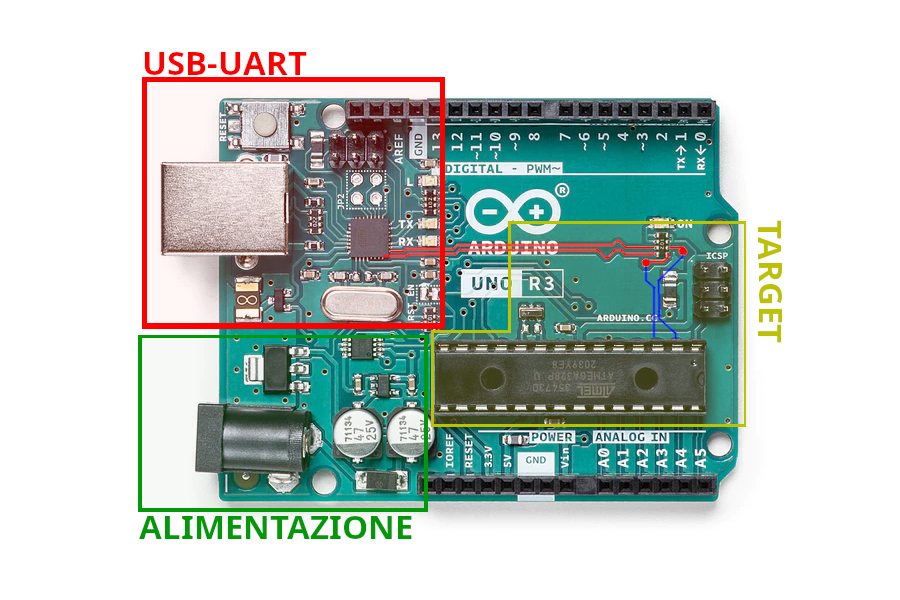
\includegraphics[width=\textwidth]{arduino-uno.png}
            \end{figure}    
        \end{minipage}
    \end{frame}
    

    \begin{frame}
        \frametitle{Problematiche comuni}
        \begin{itemize}
            \item[] <1-> Spesso il software non funziona come dovrebbe per errori logici derivati dalla complessità del linguaggio di programmazione.
            \item[] <2-> Non vi è modo di interagire con il controllore durante l'esecuzione del codice
            \item[] <3-> Si è portati ad aggiungere statement di log per individuare il problema.

        \end{itemize}

        \begin{figure}
            \begin{tikzpicture}
                \node[inner sep=0pt, label={left:1. Codifica}] (russell) at (0,0) {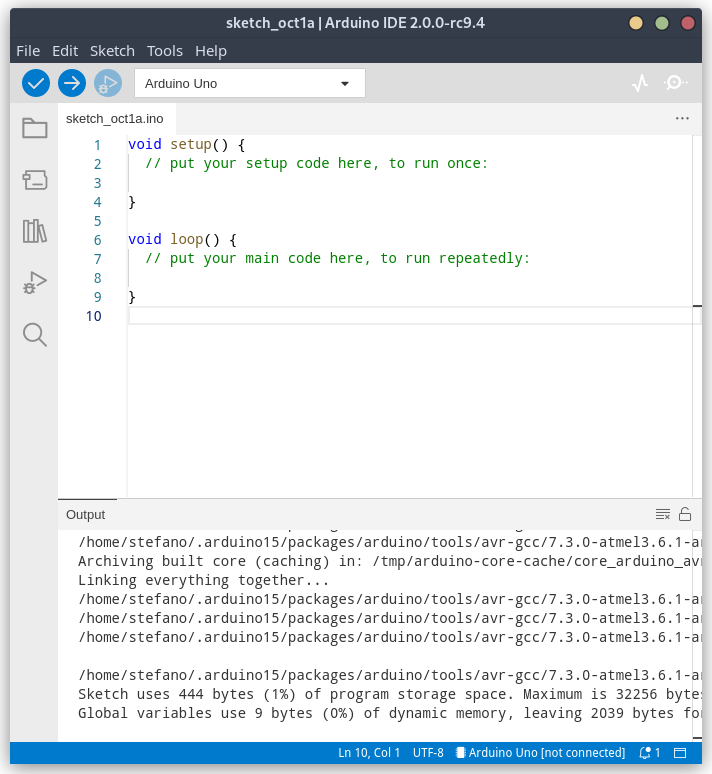
\includegraphics[width=.15\textwidth]{arduino-ide.png}};

                \node[inner sep=0pt, label={right:3. Test}] (arduino) at (5,0) {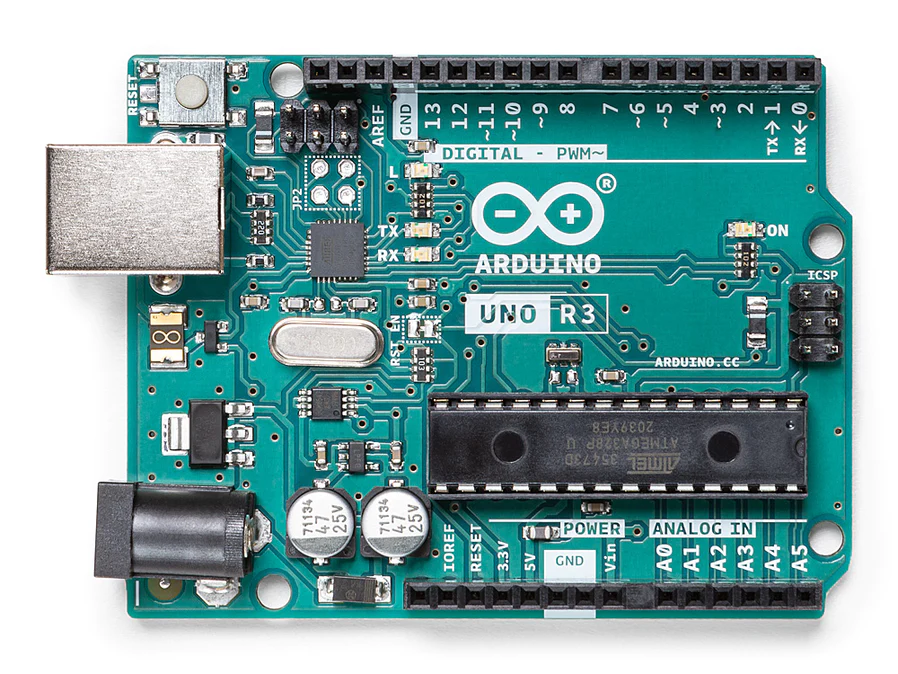
\includegraphics[width=.15\textwidth]{arduino-no-annotations.png}};

                \draw [-stealth] (0,1.2) to[bend left] (5, 0.8) ;
                \draw [-stealth] (5, -0.8) to[bend left] (0,-1.2);

                \node (0) at (2.5,1.5) [label={above:2. Caricamento}] {};
                \node (1) at (2.5,-1.5) [label={below:4. \texttt{Serial.println()}}] {};
                
            \end{tikzpicture}
        \end{figure}
    \end{frame}

    \begin{frame}
        \frametitle{Architettura GDB}
    
        \begin{itemize}
            \item[] <1-> GDB è un software di \textit{debugging} multi-architettura
            \item[] <2-> Permette di lavorare su un processo remoto tramite l'architettura client-server
        \end{itemize}

        \begin{figure}
            \begin{tikzpicture}
                \draw[fill=green!50] (0,0) rectangle (2,2) node[pos=.5] {Client GDB};
                \draw[fill=yellow!50] (5,0.5) rectangle (8,1.5) node[pos=.5] {Server GDB};
                \draw[fill=blue!50] (11,0.5) rectangle (12.5,1.5) node[pos=.5] {\textit{target}};

                \draw [stealth-stealth](2,1) -- (5,1) node[label={[font=\footnotesize]above:Protocollo GDB},pos=.5] {};
                \draw [stealth-stealth](8,1) -- (11,1) node[label={[font=\footnotesize]above:DebugWire\cite{site:dw-reverse-engeneering}},pos=.5] {};
            \end{tikzpicture}
        \end{figure}
    \end{frame}
    \note{
        È possibile notare la similitudine con l'architettura host-programmatore-target
    }
    
    \begin{frame}
        \frametitle{Implementazione \hfill 1}
    
        \begin{figure}
            \begin{tikzpicture}[scale=0.80]
                \draw[fill=green!50] (0,3) rectangle (4,4) node[pos=.5] {GDB}; %GDB
                \draw[fill=yellow!50] (0,2) rectangle (4,3) node[pos=.5] {GDB proto}; %gdb_proto
                \draw[fill=red!50] (0,1) rectangle (4,2) node[pos=.5] {CDC}; %cdc
                \draw[fill=blue!50] (0,0) rectangle (4,1) node[pos=.5] {USB PHY}; %usb_phy
                
                \draw[fill=purple!50,purple!50,text=black] (5,3) rectangle (9,4) node[pos=.5] {GDB server}; %GDB_SERVER
                \draw[fill=purple!50,purple!50] (7.5,2) rectangle (9,3); 
                \draw (5,3) -- (5,4) -- (9,4) -- (9,2);
                \draw[fill=yellow] (7.75,2) rectangle (8.75,2.5) node[pos=.5] {RTT}; %RTT
        
                \draw[fill=yellow!50] (5,2) rectangle (7.5,3) node[pos=.5] {GDB proto}; %gdb_proto
                \draw[fill=red!50] (5,1) rectangle (7.5,2) node[pos=.5] {CDC}; %cdc
                \draw[fill=blue!50] (5,0) rectangle (7.5,1) node[pos=.5] {USB PHY}; %usb_phy
                \draw[fill=gray!50] (7.5,1) rectangle (9,2) node[pos=.5] {dW}; %dw
                \draw[fill=orange!50] (7.5,0) rectangle (9,1) node[pos=.5] {UART}; %uart
        
                \draw[fill=cyan!50] (10,2) rectangle (14,3) node[pos=.5] {Process}; %AVR
                \draw[fill=yellow] (12.75,2) rectangle (13.75,2.5) node[pos=.5] {RTT}; %RTT
                \draw[fill=gray!50] (10,1) rectangle (14,2) node[pos=.5] {dW}; %dw
                \draw[fill=orange!50] (10,0) rectangle (14,1) node[pos=.5] {UART (O.D.)}; %UART
        
                \draw[black, thick] (2, 0) -- (2, -0.5) -- (6.25, -0.5) -- (6.25, 0);
                \draw[black, thick] (8.5,0) -- (8.5, -0.5) -- (12, -0.5) -- (12, 0);
        
                \node (5) at (2, 4.5) {Host};
                \node (5) at (7, 4.5) {Adapter};
                \node (5) at (12, 4.5) {Tagret (AVR)};
            \end{tikzpicture}
        \end{figure}
    \end{frame}

    \begin{frame}
        \frametitle{Implementazione \hfill 2}
    
        \begin{figure}
            \begin{tikzpicture}
                \node[inner sep=0pt] (arduino) at (0,0) {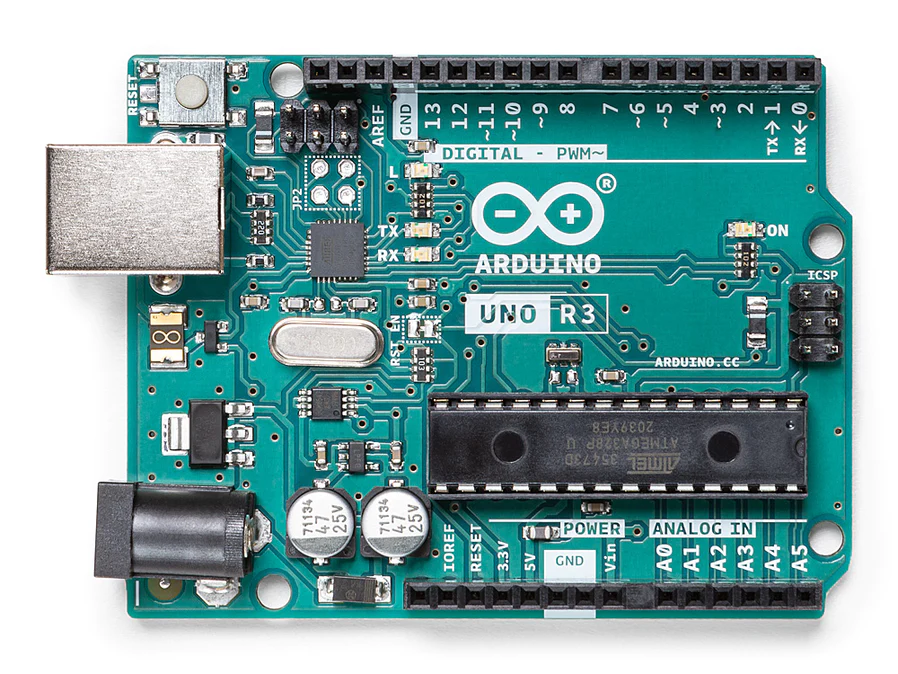
\includegraphics[width=.5\textwidth]{arduino-no-annotations.png}};

                \draw [fill=green!50] (-8, 0) rectangle (-6, 2) node [pos=.5] {Host};
                \draw [fill=yellow!50] (-1.1, 0.45) rectangle (-0.65, 0.88) node [pos=.5] {A};
                \draw [fill=blue!50] (2.75, -0.55) rectangle (-0.15, -1.15) node [pos=.5] {Target};

                \draw [semithick] (-6, 1) -- (-3.1, 1);
                \draw [color=yellow, thick] (-1.8, 1) -- (-1.45, 1) -- (-1.235, 0.665) -- (-1.1, 0.665);
                \draw [color=red, thick] (-0.65, 0.665) -- (2.3, 0.665) -- (2.5, 0.465) -- (2.5, -0.3) -- (2.7, -0.5);
            \end{tikzpicture}
        \end{figure}
    \end{frame}

    \begin{frame}
        \frametitle{Modifiche hardware}
        \begin{minipage}{.55\textwidth}
            Al fine di rendere la scheda compatibile con il protocollo debug wire:
            \begin{itemize}
                \item <1-> È stato rimosso il condensatore che isolava la connessione tra il pin dell'integrato adattatore e controllore target
                \item <2->  Sono state isolate alcune resistenza di pull-down
                \item <3->  È stato isolato il pulsante di reset
            \end{itemize}
        \end{minipage}
        \begin{minipage}{.44\textwidth}
            \begin{figure}
                \hfill
                \begin{minipage}{.45\textwidth}
                    \subfloat[][]{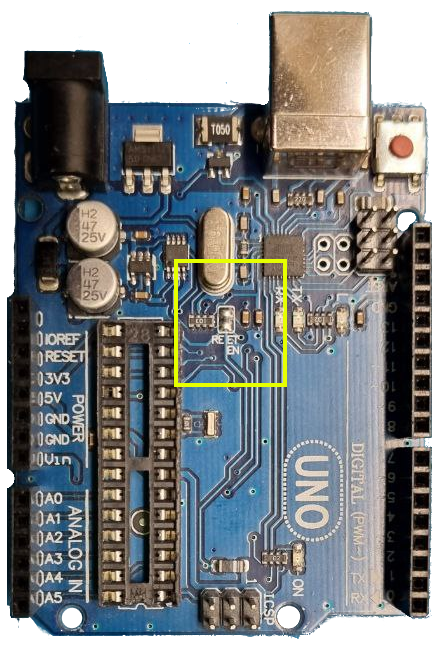
\includegraphics[width=.9\textwidth]{cap_begin.png}}
                \end{minipage}
                \begin{minipage}{.45\textwidth}
                    \subfloat[][]{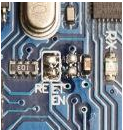
\includegraphics[width=.5\textwidth]{cap_removed.png}} \\
                    \subfloat[][]{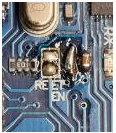
\includegraphics[width=.5\textwidth]{cap_shorted.png}}
                \end{minipage}
                \hfill
            \end{figure}
        \end{minipage}
    
    \end{frame}

    \begin{frame}
        \frametitle{Risultati}
        
        \begin{figure}
            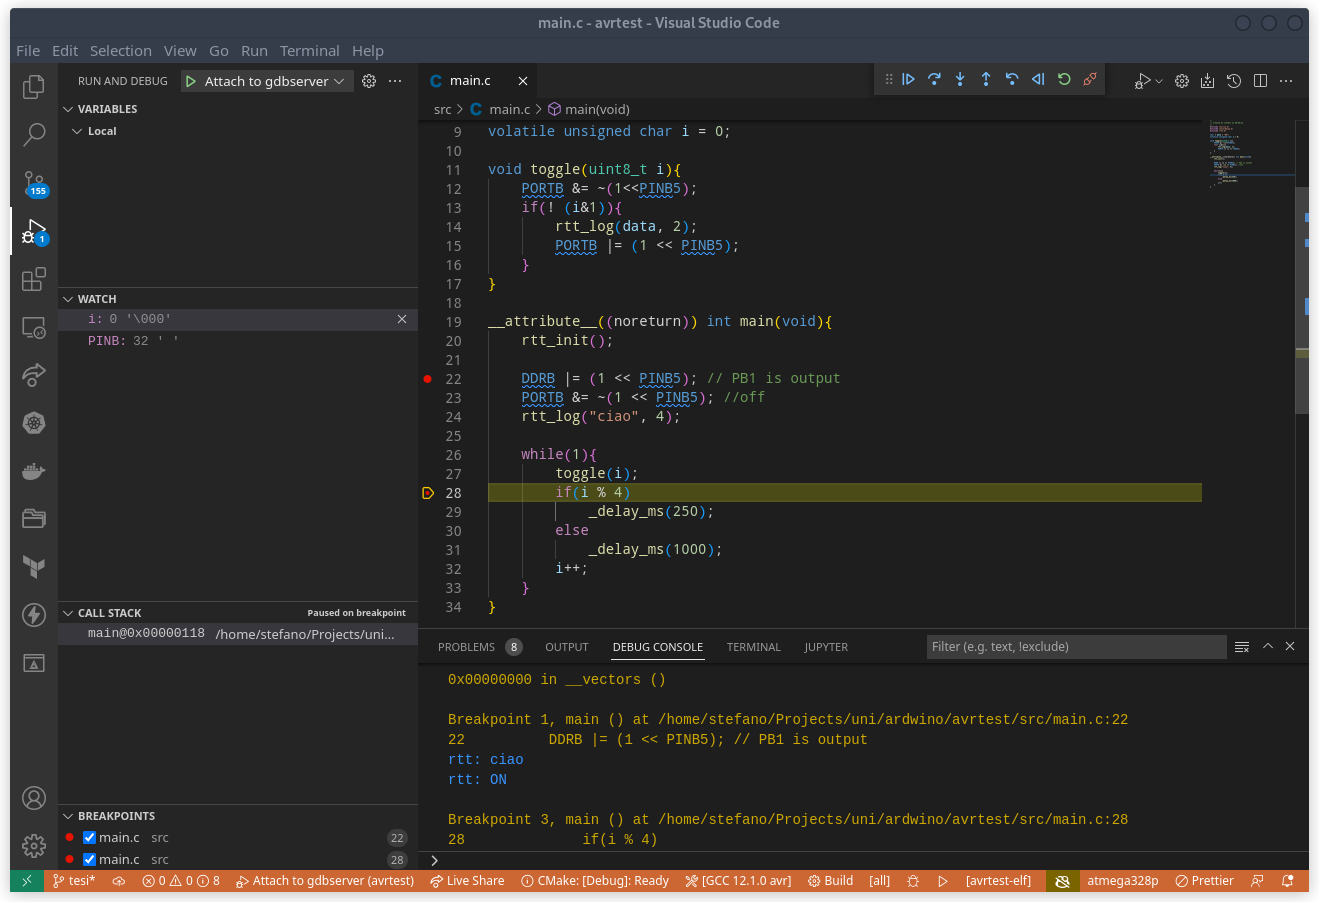
\includegraphics[height=.7\textheight]{vscode-dbg.png}
        \end{figure}
    
    \end{frame}

    \begin{frame}
        \frametitle{Bibliografia e Sitografia}
        \printbibliography[heading=none]%
    \end{frame}

    \begin{frame}
    \end{frame}

\end{document}
